\section{Black Holes}
\subsection{Formation of Black Holes}
Black holes can form when massive stars collapse under their own gravity at the end of their life cycles.
\subsection{Event Horizons}
The event horizon is the boundary beyond which light and other signals cannot escape to distant observers.

The Event Horizon Telescope collaboration published an image of the black hole shadow in the galaxy M87 \parencite{eventhorizon2019}.

\begin{figure}[htbp]
    \centering
    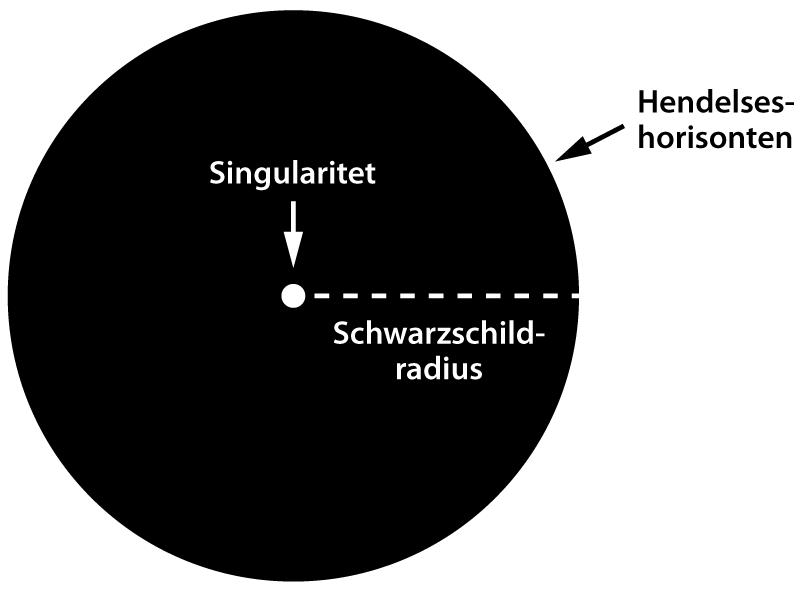
\includegraphics[width=0.75\textwidth]{figures/images/black-hole-diagram.png}
    \caption{Simplified schematic of a black hole and its event horizon.}
    \label{fig:black-hole}
\end{figure}

The Schwarzschild radius is denoted by $r_s$ and depends on the mass $M$ of the object.

\[
r_s = \frac{2GM}{c^2}
\]